\documentclass[handout]{beamer}
\usepackage[french]{babel}
\usepackage[T1]{fontenc}
\usepackage[utf8]{inputenc}
\usepackage{graphicx}
\usepackage{subfig}
\usepackage{epstopdf}
% functions to plot
\def\func(#1){(#1)*(1-(#1))}
\hypersetup{colorlinks = true,linkcolor = blue,urlcolor  = blue}

\newcommand{\qGraph}[1]{\begin{center} \includegraphics[width =
0.6\textwidth]{#1}\end{center}}

\newenvironment{iPar}[1]{\textbf{#1} \begin{itemize}}{\end{itemize}}

\newcommand{\inc}{{inc}}
\newcommand{\cp}{{cmp}}
\newcommand{\bull}{$\bullet\;$} 

\newcommand{\esp}{\mathbf{E}} \newcommand{\ul}[1]{\underline{#1}}
\newcommand{\ol}[1]{\overline{#1}} \newcommand{\ora}[1]{\textbf{#1}}

\addtobeamertemplate{navigation symbols}{}{%
    \usebeamerfont{footline}%
    \usebeamercolor[fg]{footline}%
    \hspace{1em}%
    \insertframenumber/\inserttotalframenumber
}

\newcommand{\mdp}{\medskip \pause}

\title{Price and Income Effects}
\author{Microeconomics \\ 20851}
\date{}

\begin{document}

\frame{\titlepage}

\section[Outline]{}
\frame{\tableofcontents}

\begin{frame}{Does a Tax on Fuel Promote Public Transit?}
\begin{figure}
\subfloat[price effect]{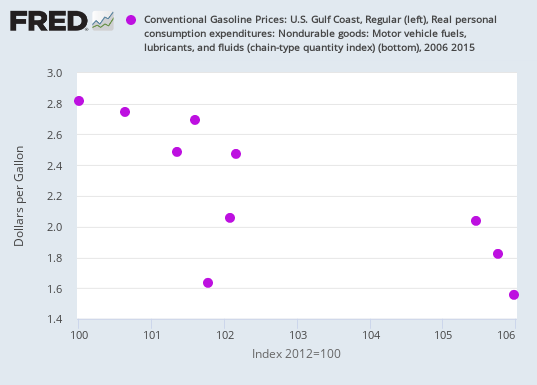
\includegraphics[scale=0.185]{price.png}}
\subfloat[income effect]{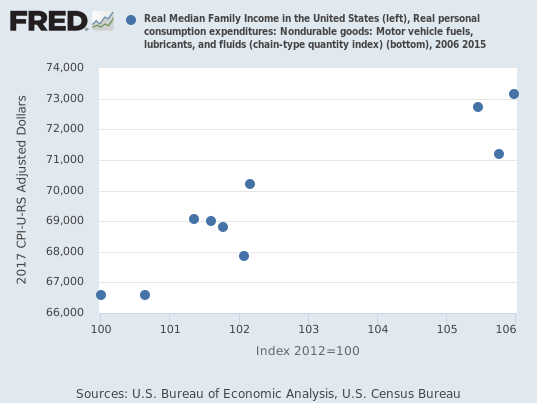
\includegraphics[scale=0.18]{income.png}} 
\subfloat[cross effect]{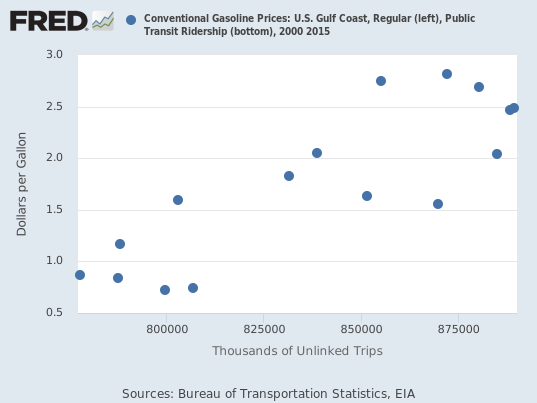
\includegraphics[scale=0.18]{transit.png}}
\caption{FRED Data on fuel price and consumption and public transit}
\end{figure}


\end{frame}

\section{Price and Income Effects}

\begin{frame}\frametitle{Demand Preferences}
\textbf{The problem}
\begin{itemize}
\item Fuel (X) and Public Transit (Y)
\item Utility $U(X,Y)$
\item Budgand constraint: $p_X Y+ p_Y Y = I$
\end{itemize}

\textbf{Optimizing with a given constraint:}
\begin{itemize}
\item  $(X^*, Y^*)$ such that \begin{eqnarray*} \frac{dU}{dX}\Bigg/\frac{dU}{dY} = \frac{p_X}{p_Y} \textrm{ and }
p_X X + p_Y Y = I
\end{eqnarray*}

\item  At the optimum: the budget  is respected and we are indifferent between giving up some $X$ to acquire $Y$ and vice versa.
\item Two equations, two variables: we can solve for $X^*$ and $Y^*$ as a function of $(p_X,p_Y,I)$

\end{itemize}
\end{frame}

\begin{frame}{Example}
\begin{itemize}
\item $U(X,Y) = \ln X +  2\ln Y$ \pause
\begin{eqnarray*}\frac{dU}{dX}\Bigg/\frac{dU}{dY} &=& \frac{p_X}{p_Y} \iff \frac{1/X}{2/Y} = \frac{p_X}{p_Y} \\ \iff  p_Y Y = 2p_X X \end{eqnarray*}
\item With $p_X X + p_Y Y =  I$ implies $$X^* = \frac{I}{3p_X} \textrm{ and } Y^* = \frac{2I}{3p_Y}$$

\end{itemize}
\end{frame}


\begin{frame}{How $X^*$ and $Y^*$ Vary as a Function of $I$}
\begin{iPar}{Engel's curve}
\item Individual demands  $X(p_X,p_Y,I)$, $Y(p_X,p_Y,I)$.
\item Engel's curve for $X$: how does $X^*$ change when $I$ changes
\item Proportion of the budget dedicated to $X$: $s_X = \frac{p_X X}{I}$
\end{iPar} 

\begin{iPar}{Normal goods}
\item A good is said to be normal if and only if the demand of the good increases with income (constant prices)
\item Example: fuel (luxury car)
\end{iPar}

\begin{iPar}{Inferior goods}
\item A good is said to be inferior if demand decreases as income increases (constant prices)
\item Example:  it depends on initial income levels, but junk food (kraft dinner), lottery tickets, perhaps public transit?
\end{iPar}

\end{frame}

\begin{frame}{How the Demands $X^*$ and $Y^*$ Change with Prices}
Keep $p_Y$ and $I$ constant. How does the demand adjust to an increase of $p_X$? 

\end{frame}

\begin{frame}{Decomposing Demand Changes}
When fuel price $p_X$ increases, two forcess: \begin{itemize}
\item Public transit is more affordable than a car (fuel): Want to consume more of the cheaper good. This is the \textbf{substitution effect}. $$ \frac{U'_X(X,Y)}{U'_Y(X,Y)} = \frac{p_X}{p_Y}$$

\item Purchasing power decreases: need more income to by the same basket of goods as before the change: \textbf{income effect}.
\end{itemize}

\textbf{Objective:} Identify price effects and income effects

\end{frame}

\begin{frame}{Compensated Demand}

\begin{iPar}{Context}
\item Reference price $(p_X,p_Y)$, Reference income $I$, new price $(\hat p_X,p_Y)$
\item Reference demand, $X(p_X,p_Y,I)$, reference (indirect) utility $V(p_X,p_Y,I)$
\item New demand, $X(\hat p_X, p_Y, I)$, new (indirect) utility $V(\hat p_X,p_Y,I)$.
\end{iPar}
\end{frame}

\begin{frame}{Compensated Demand}
\begin{iPar}{Definition}
\item Compensated income: income $I^\cp$ such that we can achieve the reference utility with the new prices $$V(p_X,p_Y, I) = V(\hat p_X, p_Y,  I^\cp)$$
\item Compensated demand $X^\cp = X(\hat p_X, p_Y,  I^\cp)$
\item \textbf{Property:}  IF $\hat p_X > p_X$, then $X^\cp <X(p_X,p_Y,I)$\\ the compensated demand of $X$ is decreasing in terms of $p_X$.
\end{iPar}
\end{frame}

\begin{frame}{Compensated Demand}

\textbf{Exercise A}: Calculate the compensated income and demand for $X$ if $U(X,Y) = XY$ and $p_XX+p_YY \le I$ for a price change $\hat p_X > p_X$. 

\end{frame}



\begin{frame}{Substitution and Income Effects}

\begin{iPar}{Substitution effect}
\item  Change in demand caused by relative price change, keeping utility constant:
\item Substitution Effect $=$ Compensated demand - Reference demand

$$ \Delta X^{\cp} =  X(\hat p_X,p_Y,I^\cp) - X(p_X,p_Y,I) $$

\end{iPar}

\begin{iPar}{Income effect}
\item  A change in demand caused by a change in purchasing power keeping prices constant
\item Income effect $=$ New demand - Compensated demand
\end{iPar}
$$ \Delta X^{I} = X(\hat p_X,p_Y,I) - X(\hat p_X,p_Y,I^\cp) $$

\end{frame}

\begin{frame}{Approximating the Compensated Income}
Consider a small price change $\hat p_X = p_X + \Delta p_X$. To keep notation simple: $X^* = X(p_X,p_X,I)$, $Y^* = Y(p_X,p_Y,I)$\\ \smallskip

We define $I^\cp  = I + \Delta I^\cp$, $X^\cp = X^* + \Delta X^\cp$ and  $Y^\cp  = Y^* + \Delta Y^\cp$.

\begin{align*}
I^\cp & =  \hat p_X X^\cp +  p_Y Y^\cp\\
 & =  (p_X + \Delta p_X)(X^* + \Delta X^\cp) + p_Y(Y^* + \Delta Y^\cp)\\ 
  &=  \underbrace{p_X X^* + p_YY^*}_{=I} +\underbrace{\Delta p_X \Delta X^\cp}_{\simeq 0} + \Delta p_X X^* \\
  & \quad \quad \quad + \underbrace{ p_X\Delta X^{\cp} + p_Y \Delta Y^{\cp}}_{=0}\\ & \simeq I+  \Delta p_X X^* \\
 \Delta I^\cp  &\simeq \Delta p_X X^*
\end{align*}
\end{frame}

\begin{frame}{A Trick to identify Compensated Income}

Why does $p_X\Delta X^{\cp} + p_Y \Delta Y^{\cp} = 0$?

\begin{enumerate}
\item $(X^*,Y^*)$ and $(X^\cp,Y^\cp)$ are on the same indifference curve, which implies $$\frac{\Delta Y^\cp}{\Delta X^\cp} = MRS_{X\to Y} $$
\item $(X^*,Y^*)$ is optimal at the prices $p_X, p_Y$, which implies $MRS_{X\to Y} = -\frac{p_X}{p_Y}$.
\item Therefore, $p_X \Delta X^\cp + p_Y \Delta Y^\cp = 0 $.
\end{enumerate}

\textbf{Exercise B}: Check if this approximation works for $U(X,Y) = XY$ with reference prices and income $(p_X,p_Y,I) = (1,1,100)$ and $\Delta p_X = 1$ and $\Delta p_X = 0.1$.
\end{frame}

\begin{frame}{The Slutsky Equation}
This equation comes from the decomposition of the price elasticity of demand.\medskip

To keep notation simple, consider 
\begin{align*}
 X^* &= X(p_X,p_Y,I), &     X(p_X + \Delta p_X, p_Y,I) &= X^* + \Delta X^*,\\ && X(p_X + \Delta p_X, p_Y,I) &= X^\cp +\Delta X^I
\end{align*}

We get
\begin{align*}
\underbrace{\Delta X^*}_{\text{Total effect}} = \underbrace{\Delta X^\cp}_{\text{Substitution effect}} + \underbrace{\Delta X^I}_{\text{Income effect}}
\end{align*}

\textbf{Exercise D}: Find the income and substitution effects in exercise C.
\end{frame}


\begin{frame}{The Slutsky Equation}
Since $$\Delta X^I =   -\frac{\partial X}{\partial I} \Delta I^\cp =  -\frac{\partial X}{\partial I}  \Delta p_X X^*$$
Then,
\begin{align*}
\Delta X^* &=   \underbrace{\Delta X^{\cp}}_{\leq 0} -   \underbrace{\frac{\partial X}{\partial I}\times \Delta p_X X^*}_{\geq 0 \text{ if normal, } <0 \text{ if inferior}} 
\end{align*}
As an elasticity, 
\begin{align*}
\frac{\Delta X^*}{\Delta p_X}\frac{p_X}{X^*} & = \frac{\Delta X^\cp}{\Delta p_X}\frac{p_X}{X^*} - \frac{\partial X}{\partial I} \Delta p_X X^*\times\frac{p_X}{\Delta p_X X^*}\frac{I}{I} 
\end{align*}
The Slutsky equation is given by: 

$$\eta_{X,p} and = \eta^\cp_{X,p}  - \eta_{X,I} \times s_X $$

\end{frame}

\section{Properties of Demand Functions}

\begin{frame}{The nature of goods}

The goods $X$ and $Y$ are:
\begin{itemize}
\item Substitutes: if the cross effect is $\frac{\partial X^\cp}{\partial p_Y} >0$
\item Compléments: if the cross effect is $\frac{\partial X^\cp}{\partial p_Y} <0$ 
\end{itemize}

\end{frame}

\begin{frame}{Properties}

\begin{itemize}
\item Homogeneity of degree 0 $$X(\lambda p_X,\lambda p_Y,\lambda I) = X(p_X,p_Y,I)$$ 
\item Symetry: $$\frac{\partial X^\cp}{\partial p_Y} =\frac{\partial Y^\cp}{\partial p_X} $$ 
\item Additivity: $$ p_X \frac{\partial X(p_X,p_Y,I)}{\partial I} + p_Y \frac{\partial Y(p_X,p_Y,I)}{\partial I} = 0 $$
\item Negativity: $$\frac{\partial X^\cp}{\partial p_X}<0,\frac{\partial Y^\cp}{\partial p_Y}<0$$

\end{itemize}

\end{frame}

\section{Special Cases}

\begin{frame}{Giffen Goods}
\begin{iPar}{Direction of income and wealth effects}
\item When indifference curves are convex, the compensated demand for $X$ decreases as $p_X$ increases
\item Income effects depend on whether the good is normal or inferior at reference income and prices.
\item If normal good, price increase causes a negative income effect (same direction as price effect)
\item If inferior good, price increase causes a positive income effect (opposite direction)
\end{iPar}

\begin{iPar}{Giffen Goods}
\item If the income effect is larger than the substitution effect, as the price $p_X$ increases, the demand for $X$ increases.
\item  Classic example : Potatoes in Ireland (circa 1850, according to legend). 
\end{iPar}
\end{frame}

\begin{frame}{Chinese Rice Subsidy}

\begin{figure}
\subfloat{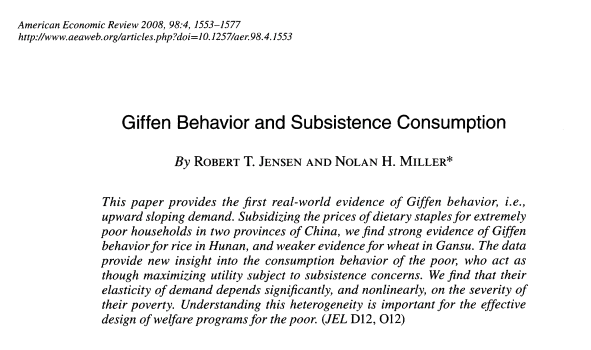
\includegraphics[scale=0.3]{china.png}}
\subfloat{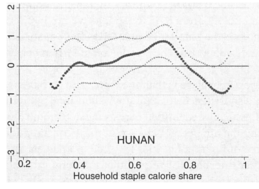
\includegraphics[scale=0.5]{elasticity_share.png}}
\end{figure}

\end{frame}

\begin{frame}{Doctors}
How can a wage increase cause a drop in work hours?
\begin{figure}
\centering

\includegraphics[scale=0.2]{docteurs.png}
\caption{\href{https://www.tvanouvelles.ca/2018/05/17/medecins-de-familles-la-moitie-travaillent-4-jours-et-moins}{TVA Nouvelles}}
\end{figure}
\end{frame}

\begin{frame}{Price and Costs of Living Indexes}

To measure changes in costs of living, we often use consumption price indices. A very common one is the Laspeyres index: 

$$ \pi_L = \frac{\hat p_X X + \hat p_Y Y}{p_X X + p_Y Y} $$

\begin{itemize}
\item The Quebec Pension Plan (QPP) and private pension plans are often indexed using this kind of index.
\item Is this a good index to capture an increase in the cost of living?

\end{itemize}

\end{frame}

\begin{frame}{The Ideal Price Index}

Need account for behavioral changes. Therefore, a price increases implies substitution. 

\begin{itemize}
\item Following a price increase for the good $X$, the necessary compensation to keep welfare constant is 

$$ \pi_I =  \frac{I^{cmp}}{I} $$.

\item In a Cobb-Douglas situation $u(X,Y)=X^{\alpha}Y^{1-\alpha}$: 

$$ \pi_I = \frac{I^{cmp}}{I} = \left(\frac{\hat p_X}{p_X}\right)^\alpha$$

\end{itemize}

\end{frame}

\end{document}




